\chapter{Aneka}
\section{Introduction}
Aneka is a Platform-as-a-Service (PaaS) that enables the development of distributed applications for use across a broad range of cloud, grid and cluster platforms. Originally developed as part of the Gridbus Project, Aneka was later commercialised by Manjrasoft and is developed on top of .NET technology. It is available freely for a trial period\ftAnone, however additional arrangements must be made for commercial use. Aneka allows for applications to be developed in any language that is supported by the .NET runtime, such as VB.NET and C\#, and through the use of Mono, allows applications to run on Linux and OSX as well as Windows infrastructures\cite{Aneka}.
\ftAnoneText

\begin{center}
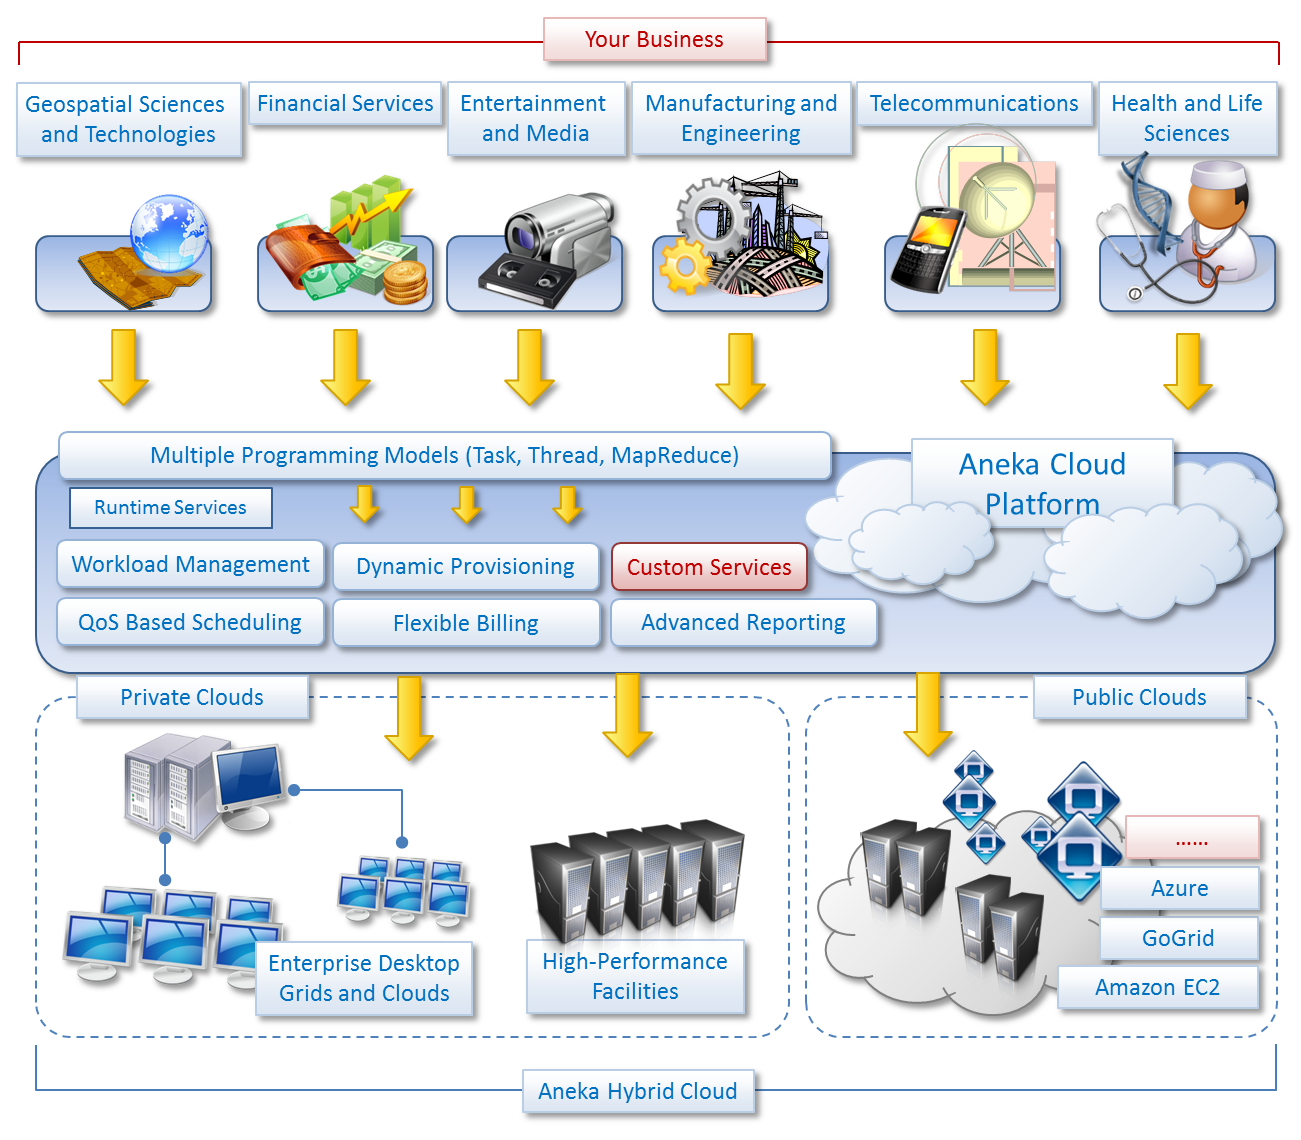
\includegraphics[scale=0.6]{figs/Aneka.png} \\
\texttt{Architecture of Aneka Platform}\ftAntwo\ftAntwoText
\end{center}


\section{Platform as a Service}
PaaS solutions, such as Aneka, provide a platform from which distributed applications can be developed that scale on demand\cite{CloudBus}. Aneka is a pure PaaS in that it does not provide an underlying hardware infrastructure. This differs from other PaaS solutions such as Google AppEngine and Microsoft Azure, which are both PaaS and Infrastructure-as-a-Service (IaaS) solutions. Instead, Aneka is designed to work as a platform layer on top of a variety of infrastructures, including combinations of multiple different options. This allows for the use of local resources when available, with the added ability for the provision of additional cloud resources from a service such as Amazon EC2 when the required job is unable to be completed on the local infrastructure within the required deadline. The other combined PaaS/IaaS solutions are also tied to their respective IaaS, giving Aneka the added benefit of being able to more freely swap between IaaS providers to meet changing resource demands.

\section{Programming Models}
One of the key strengths of Aneka is its flexibility, providing three different programming models (Task, Thread and MapReduce), which has enabled the use of Aneka in a broad range of applications in the fields of Engineering, Education and the Life Sciences.
\begin{itemize}
\item The Task Programming Model is best suited to programs that are ``embarrassingly-parallel'' as tasks are handled entire independently with no restriction on their execution order\ftAnthree.
\ftAnthreeText

\item The Thread Programming Model is best suited to porting existing threaded applications to a distributed computing environment, treating each thread as a task that is distributed across the available resources in the Aneka network\ftAnfour.
\ftAnfourText

\item The MapReduce Programming Model is best suited to applications working on large datasets. Through the definition of \emph{map} and \emph{reduce} functions, Aneka will distribute the data across available resources, apply the map function and then reduce the output\ftAnfive.
\ftAnfiveText
\end{itemize}

In addition to a broad range of existing functionality, Aneka has a layered and modular software architecture which enables additional programming models and services to be developed and plugged into Aneka easily.

Each programming model is based on the abstraction of job execution into 4 distinct parts: the Work Unit, the Manager, the Executor and the Scheduler. The Work Unit is dependent on the programming model being used and, for example, could be an entire Task or a single Thread. The Manager is the application that the user interacts with, to submit jobs to the Aneka system and to collect their results at the end. The Scheduler is what organises the communication inside the Aneka system. It schedules each work unit and then packages and dispatches the applications required along with any required input files. It is also responsible for collecting the results from each node and making it available to the Manager. The Executor is node specific and is tasked with running the specific application given to it by the Scheduler\cite{Aneka}.

\section{Deployment Model}
Aneka was specially designed on top of the ECMA 335 specification, which is a Common Language Infrastructure (CLI), giving it great portability for use in heterogeneous network environments. This allows for the use of Aneka on existing physical hardware, even taking advantage of dead cycles on desktop machines, as well as allows for Aneka to be plugged transparently into external third party services such as Amazon EC2. Aneka provides a Platform Abstraction Layer (PAL) in order to help develop distributed programs that can take advantage of this CLI. The PAL provides a platform independent interface to a range of actions that would otherwise have to be platform specific, such as when it is required to interact with the hardware of the machine or accessing properties of the Operating System of the node being used.

Both programs that are specifically written to work with Aneka and existing applications are supported, though existing applications may be limited or work less effectively than if they had been modified. For existing applications, even provides a Parameter Sweeping services which will take a given application and a set of parameters and will run the application with all possible combinations of the given parameters with each combination handled by the system as an independent job and has resources allocated accordingly.

\section{Quality of Service / Service Level Agreements}
An important component of distributed computing is the ability to define requirements of Quality of Service (QoS) and Service Level Agreements (SLA)\cite{CloudBus}. Aneka provides an easy to use management tool that can negotiate specified QoS and SLA requirements with the system, and can be used to bring in additional resources in order to meet these agreements. Aneka additionally has a counter-offer service, whereby if a job cannot be completed within the requested resource limitations, an offer will be made by the system stating the minimum resources it can complete the job it.

\section{Additional Services}
Aneka provides a number of additional features including handling of billing, dynamic scheduling, workload management and advanced reporting. Reporting allows users of Aneka to closely monitor what is going on within the system, as well as providing billing functionality to charge each user of the system for their usage. The use of dynamic scheduling and workload management allows for the automatic scaling of the Aneka system as workload calls for it, providing flexible and automatic scaling to external cloud services such as Amazon EC2, Windows Azure and GoGrid Cloud Service.
